\documentclass[english, LaM, oneside]{sapthesis}%remove "english" for a thesis written in Italian
%Bachelor's (laurea triennale) thesis : Lau 
%Master's (laurea specialistica) thesis: LaM 
%PhD's thesis: PhD 
%\usepackage[italian]{babel} %use this package for a thesis written in Italian
\usepackage[utf8]{inputenx}
\usepackage{indentfirst}
\usepackage{microtype}
\usepackage{pdfpages}
\usepackage{graphicx}
%\usepackage{chemformula}
%\usepackage{setspace}
%\usepackage{yfonts,color}
%\usepackage{siunitx}
%\usepackage{comment}
%\usepackage{multirow}
%\usepackage{varioref}
%\usepackage[bottom]{footmisc}
%\usepackage{wrapfig}
%\usepackage{float}
%\usepackage{type1cm}
\usepackage{lettrine}
\linespread{2}
%\usepackage{chngcntr}
\usepackage[nottoc, notlof, notlot]{tocbibind}
%\onehalfspacing
%\counterwithout{footnote}{chapter}
\usepackage{hyperref}
\hypersetup{
			hyperfootnotes=true,			
			bookmarks=true,			
			colorlinks=true,
			linkcolor=red,
                        linktoc=page,
			anchorcolor=black,
			citecolor=red,
			urlcolor=blue,
			pdftitle={Thesis},
			pdfauthor={FirstName LastName},
			pdfkeywords={thesis, sapienza, roma, university}
 }

\title{Design and development of rentable and \textit{layawayable} Non-Fungible Token standard for Ethereum and EVM-compatible blockchains}
\author{Andrea Palermo}
\IDnumber{1810218}
\course[]{Computer Science}
\courseorganizer{Facolt\`a di Ingegneria dell'informazione, informatica e statistica}
\submitdate{2022/2023}
\copyyear{2023}
\advisor{Prof. Claudio Di Ciccio}
%\coadvisor{Dr. co-advisor}
\authoremail{palermo.1810218@studenti.uniroma1.it}
%\examdate{X March 2023}
%\examiner{Prof. ...} \examiner{Prof. ...} \examiner{Prof. ...}  \examiner{Prof. ...}  \examiner{Prof. ...} \examiner{Prof. ...}  \examiner{Prof. ...} 

%we refer to http://ctan.mirrorcatalogs.com/macros/latex/contrib/sapthesis/sapthesis-doc.pdf for an exhaustive description of the sapthesis documentclass.


\begin{document}

\frontmatter
\maketitle

\begin{abstract}
Non-Fungible Tokens (NFTs) are digital assets that represent ownership or proof of authenticity of a unique item or piece of content, such as a piece of art, music, or video. Unlike fungible tokens (cryptocurrencies), each NFT is unique and cannot be split in sub-units or exchanged on a one-to-one basis with another token. NFTs use blockchain technology to verify ownership and authenticity, making them highly secure and resistant to counterfeiting. The popularity of NFTs has grown in recent years, leading to the creation of NFT marketplaces and the rise of NFT-based collectibles, digital art, and other types of assets (in the form of both physical and digital objects). However, one of the main challenges faced by NFT owners is the lack of liquidity. While NFTs are valuable, they cannot be easily converted into money, which limits their use and potential value.\newline
This limitation, together with the fact that assets represented as NFTs are intrinsically well suited to be rented and layawayed, led rental and layaway services to become very important sectors within the Non-Fungible Token ecosystem. These concepts allow for NFT owners to temporarily layaway or rent out their assets to others, offering a new level of liquidity and monetization capabilities for NFT holders and creating new opportunities for NFT enthusiasts to gain access to unique and valuable NFTs without having to purchase them outright.

\end{abstract}

\tableofcontents

\mainmatter
\chapter{Introduction}
\lettrine[lines=2, findent=3pt, nindent=0pt]{N}{}on-fungible tokens represent ownership of unique physical or digital assets, such as artworks or music, or even a real apartment. They are stored on a blockchain, which provides a secure and transparent record of ownership, and their usage has enabled the creation of new marketplaces and revenue streams. As the popularity of NFTs has grown, so too has the interest in alternative ways to acquire them. Two such methods are NFT rental and NFT layaway.

NFT rental is a concept similar to traditional rental arrangements, such as renting a car or a vacation home. With NFT rental, users can enjoy the benefits of owning an NFT for a limited time, without the need to make a large upfront payment or take on the long-term responsibilities of ownership.
This concept allows for NFT owners to rent out their assets for a specified period of time, during which the renter can use the NFT for their own purposes. This can include displaying the NFT in a virtual gallery, using it in a video game or gaining access to the usage of a physical asset. The renter pays a fee for the privilege of using the NFT, and the owner earns passive income from the rental.\newline

NFT layaway, on the other hand, is a payment plan that allows individuals to acquire an NFT over time. Similar to traditional layaway plans, individuals make a series of smaller payments over a set period, after which they keep ownership of the NFT. This allows individuals to spread the cost of acquiring an NFT over a longer period, making it more accessible to those who may not have the funds to purchase it outright. In fact, it is very similar to a bank loan, whith which customers can buy a good and pay for it over a certain amount time, but without needing a centralized intermediary (the bank) who loans money to the buyer. This is possible because when the layawayed asset is an NFT, the layaway can be managed by a decentralized intermediary, namely a smart contract, which has the capability of foreclosing the token from the layaway receiver if they fail to pay for it in time.\newline

Currently, the state-of-the-art token standard mainly used for building NFT collections on Ethereum blockchain is the ERC-721 standard\cite{ref:EIP721} (an interface which defines the basic functionalities of a NFT). Whereas this standard has no problems in dealing with all basic NFT operations, it doesn't define primitives to allow the temporary usage grant of tokens (namely, rental and layaway).
Thus, the aim of this work consists in designing and developing a NFT standard which extends ERC721 adding token rental and layaway capabilities.\newline

For the sake of readability, this document will focus on a concrete application scenario which is currently gaining much traction, namely the fractionalization of apartments in the form of NFTs. These tokens can represent portions of an apartment and be managed each by their potentially different owner, and represent a perfect example of how rental and layaway capabilities can improve the usage of NFTs.
We will therefore assume for simplicity that each room of the apartment is bound to a different NFT and the access to a particular room will be granted only to the owner of the token bound to the room. This can be enforced by a simple system installed on doors that retrieves the owner of the room token on-chain and then verifies that the signature of the person trying to access matches the retrieved owner; if the verification succeeds, the door will then unlock itself. Using this approach, room token owners can access in a simple and direct way to the corresponding rooms, even during a rental or a layaway.

\section{Advantages over collateral lending}
Even if there exist a lot of NFT lending services out there, the concept of on-chain lending requires the borrower to deposit a collateral, whose value is often greater than the borrowed token value, in order to be able to reimburse the lender if the borrower doesn't return the token. This is a major limitation: NFT users are not able to gain usage rights of the token without having to pay its entire value immediately. Moreover, the borrower has to constantly monitor the value of its collateral: if it becomes less than the borrowed value, the borrower gets liquidated, incurring in a so called liquidation fee; the liquidation consists in the borrowed token being returned to the lender, and the collateral (minus the liquidation fee) being returned to the borrower. The liquidation fee is needed to pay for bots who monitor and execute liquidations and sometimes also to sustain the rental protocol.\newline
These limitations make rental and layaway much preferrable to lending with collateral, as they can grant NFT usage rights without an entire upfront payment and do not suffer liquidations risks.

\bigskip
In \hyperref[chap:1]{Chapter~\ref*{chap:1}} we  briefly describe the current state of the art in the fields of NFT layaway and rental and its limitations.

\bigskip
In \hyperref[chap:2]{Chapter~\ref*{chap:2}} we show our proposed solution, summarizing its advantages over the state of the art and describing its structure and architecture in depth.

\chapter{State of the art}
\label{chap:1} 
In this chapter we will showcase some of the existing implementations of rental and layaway services in the Ethereum ecosystem. Most of these solutions do not use a common standard, although there exists a standard approved by the Ethereum community for NFT rental, which we will discuss. For NFT layayway, on the other hand, there is no such standard, as far as the author knows.\newline
Concluding the chapter, we will also examine the potential limitations of the mentioned existing approaches.

\section{Rental}
\label{sec:caso}
For what concerns rental, as mentioned above, the Ethereum community has approved a token standard, named ERC4907\cite{ref:EIP4907}. This standard, as all Ethereum protocol changes or improvements, was approved in the form of an Ethereum Improvement Proposal (EIP). EIPs are submitted to the community by their authors, and get reviewed and possibly approved by an elected team of \textit{Ethereum editors}.\newline
This standard extends the ERC721 standard, the approved standard for Non Fugible Tokens on Ethereum ecosystem; standards are written in Solidity, the most common Ethereum smart contract programming language. Moreover, there exist a lot of other blockchains which can run the same smart contracts that run on Ethereum: this is possible thanks to the Ethereum Virtual Machine, which allows smart contracts bytecode to be executed on any type of machine (similarly to what JVM does for JAVA). This led many other blockchains to make use of the EVM; these chains are referred to as \textit{EVM-compatible chains}.
Thus, almost every NFT currently existing on EVM-compatible chains implements the ERC721 standard. However, ERC721 tokens lack of both rental and layaway capabilities, as they were not intended to be used as such.
As we said, ERC4907 extends ERC721 standards, with the aim of making these tokens also rentable.\newline
In order to understand how the EIP4907 authors meant to do so, we must first dive a little in the features of ERC721 NFTs. First of all, a ERC721 token has an owner, who is able to transfer the token to other accounts; the owner can also give their approval to a specific account in order to also allow it to transfer the token. ERC721 tokens are organized in so called collections: a single ERC721 contract can emit (\textit{"mint"}) various tokens, which will be part of a collection. Implementing rental services only using ERC721 capabilities is not possible, mainly because when an account owns a token they can always transfer it or change the address approved for transfers as they will, and this is not suitable for rental: there is no way to make sure that an account who temporarily owns a rented token will transfer it back at the end of the rental period. Even if an intermediary smart contract manages the rental making sure that the rental receiver approves the rented token's transfer rights to its contract's address, there is no guarantee that the receiver will not change their approval in a second moment during the rental period, causing the contract not to be able to transfer the token anymore.\newline
Of course, any smart contract programmer could come up with their own implementation of rentable NFTs which extends ERC721 standard overcoming these issues, but these solutions would not have a common standard, which would make the usage of these tokens much more complex and disorganized.\newline
EIP4907 is in fact a tentative of creating such a standard: the authors manage to do so by adding an additional role other than the token owner, called \textit{user}. The user represents the receiver of a rental, and when the rental period ends, the user gets deleted. However, this solution has some important limitations, which will be discussed at the end of the chapter.\newline
Other tentatives have been made within EVM-compatible chains in order to implement ERC721 NFTs rental without creating a new token standard. These approaches overcome the issue of the missing capabilities of ERC721 tokens mentioned above by creating a so called \textit{wrapped} version of the tokens using an intermediary contract: when some account A wants to rent a token to another account B, the intermediary contract holds the real ERC721 token in escrow for the whole rental period, giving to account B a wrapped version of the token; owning this wrapped token implies being the receiver of the rental, hence it should allow usage the token. However, this last implication is not directly guaranteed by the smart contracts, as the tokens are often used off-chain: this is the major limitation of these type of solutions, which again will be discussed at the end of the chapter.
One of the most known examples of this approach is Vera Finance\cite{ref:vera}, which offers rental and \textit{rent-to-buy} services on different EVM-compatible blockchains.


\section{Layaway}
\label{sec:caso}
NFT layaway, on the other hand, is a sector that has not currently been investigated as much as rental, and in fact lacks a standard approved in the form of an EIP. As far as the author knows, there are neither any proposed EIPs of this kind that have not been approved yet.\newline
Also for layaway, a similar issue to the one discussed above regarding rental still holds: if a token is transfered to the layaway receiver, there is no guarantee that they will pay all the agreed installments on time, and if they do not do so there is no way of foreclosing the token from them to return it to the original owner just using ERC721 functionalities.\newline
However, there are some solutions which overcome this difficulties, again using a method similar to the one seen for the rental, namely holding NFTs in an escrow account.\newline 
One example of this approach is represented by Teller Finance\cite{ref:teller}, which proposes a  particular layaway model. This is how their scheme works: after putting down a down payment of up to 50 percent of the token value, users who want to receive the layaway would be matched with a lender who can meet the other half.
The NFT would then be placed in the escrow account until the user (borrower) makes all their loan payments on time. Only when these payments have been completed, the user can receive the true ERC721 token.\newline
Another very similar example is Supermojo\cite{ref:supermojo}, which implements an analogue model.\newline
Again, the limitations of these types of approaches will be examined in the last section of the chapter.

\section{State of the art solutions' limitations}
\label{sec:caso}
In this section we will showcase the limitations of the solutions described above.\newline
For what concerns rental, we first examine Vera Financial's approach (which from now on we will denote as \textit{escrow-wrap} model). The greatest limitation of this type of solution, as hinted above, is the fact that owning the wrapped version of a NFT does not automatically guarantee its usage rights. To be more specific, concrete usage of assets bound to NFTs happens off-chain: in our apartment fractionalization setting, for instance, the rooms are obviously physical assets whose usage right is granted by granting access to them; access has to be granted by an off-chain system like the one we described, simply because a smart contract will never be able to directly act on physical or off-chain objects. This entails that the off chain usage rights granting system of assets bound to NFTs can be programmed arbitrarily by its developer: this is the reason why we can state that being the owner of a token does not \textit{automatically} grant its usage rights. Of course, what usually happens is that the off-chain platforms where the NFT assets can be used will grant usage rights to the owner of the token (as it is the role defined in ERC721 standard as the proprietor of the token). However, as we explained, this is not automatic and cannot be enforced on-chain.
Another example can be done for NFTs representing in-game assets: the videogame will allow usage of a token only to its owner.\newline
As we can easily imagine, this is an important limitation for the \textit{escrow-wrap} model, as the wrapped tokens are managed by a separate contract (different from the contract who manages the original token), so it is not likely that off-chain usage rights granting systems will take into account this different contract address in order to fetch the owner of the NFT. A possible solution would be modifying these systems in order to also check the new wrapper contracts' addresses, but it would not very suitable and straightforward, as it would have to be done for each token collection and wrapper contract separately: if an off-chain system is in charge to grant usage rights of many different ERC721 token collections, it would have to try to fetch the owner of a token from its collection's contract and each possible wrapper contract. Moreover, the list of all these wrapper contracts would not be well-defined, as any developer can come up with its own new wrapper contract at any moment. Additionally, as stated before, these type of contracts do not necessarily extend a common standard, which makes their usage quite inconvenient, as there is no standard way to use their functionalities. \newline
Other than this, there exist also other less impactful limitations of \textit{escrow-wrap} model: the wrapper and escrow contracts constitute an additional unnecessary potential point of failure other than the ERC721 contract which mints tokens; this implies that these additional contracts must gain the trust of NFT users.\newline
Moving on to the other discussed rental approach, namely EIP4907, we can examine its own limitations compared to the previously discussed ones. First of all, ERC4907 suffers a limitation similar to the one discussed for the \textit{escrow-wrap} model. In particular, the addition of the user role causes some ambiguity and retro-compatibility problems: as seen before, the off-chain platform where the NFT assets are used can arbitrarily assign usage rights to any user; this causes ambiguity when there exist more roles other than the token owner. Having the additional user role, the choice of whom should be granted usage rights is left to the off-chain platform. This can create ambiguities and also retro-compatibility issues, as before the creation of the standard only the owner role existed, hence many of the existing platform will grant usage rights to the owner, having no notion of the user.\newline
Additionally, the implementation of ERC4907 suffers some problematic implications: as it is written, it lets the owner of a rented token change the rental user and deadline at any time, and also transfer the token during the rental period, deleting the user (hence stopping the rental). This is not suited if we want the rental service to be trustless, in the sense that rental provider and receiver can use the service without having to trust each other. Using ERC4907, the receiver has to trust the provider, as they will be able to end the rental whenever they like. This is not quite appropriate, as blockchains and tokens living on them are mostly meant to be used in a trustless way (without having to trust a centralized entity).\newline
For what concerns layaway, on the other hand, we have seen that the most known existing solutions again use a \textit{escrow-wrap} model. Hence, the limitations of these approaches are analogue to the ones described for \textit{escrow-wrap} rental. Again, the platform which grants tokens' usage rights should check the tokens' ownership on all potential wrapper contracts, not necessarily in a standard way.


\chapter{Proposed solution}
\label{chap:2}
\section{Solution and advantages over state of the art}
Lorem ipsum...
\subsection{Rental}
\subsection{Layaway}

\section{UML structural and behavioral diagrams}
\label{sec:moons}
\textit{Lorem ipsum} ... \cite{ref:science}

\subsection{Class diagram}
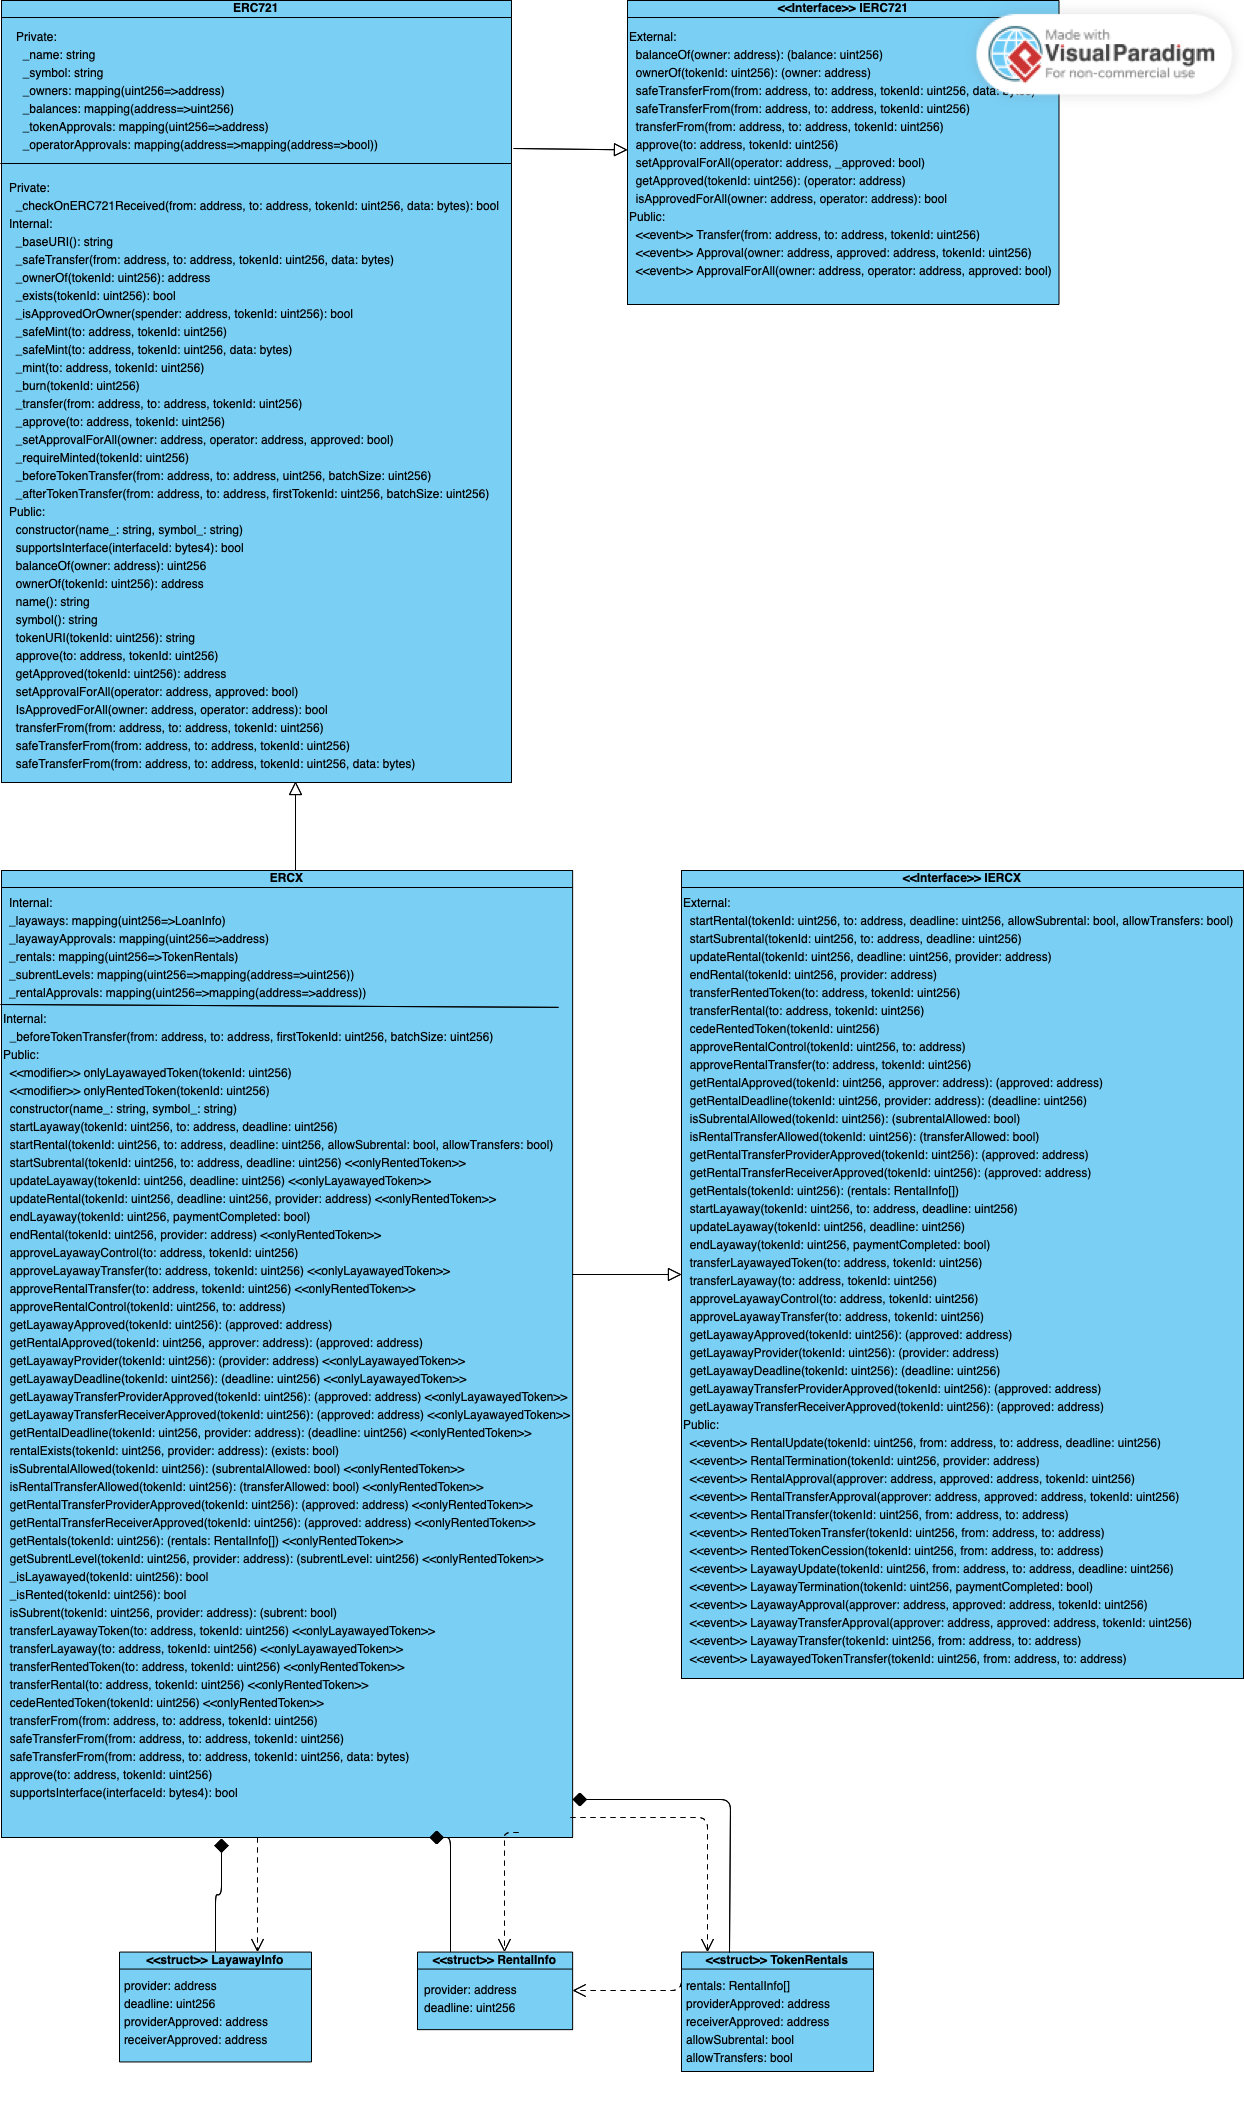
\includegraphics[scale=0.3]{classDiagram.png}
\subsection{Use cases diagram}
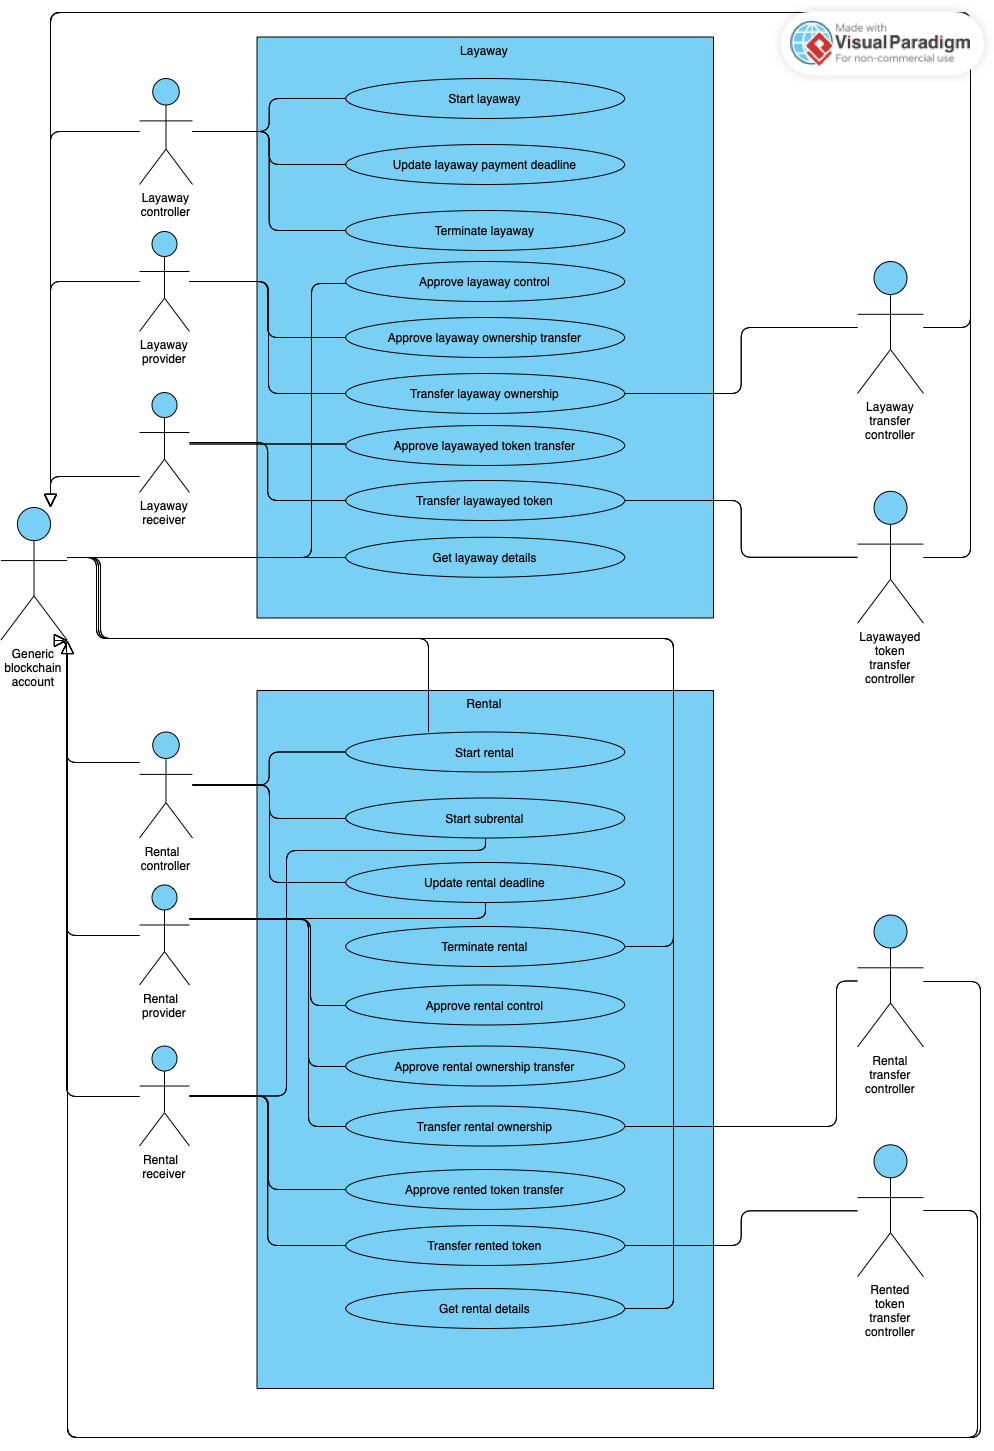
\includegraphics[scale=0.4]{useCaseDiagram.png}
\subsection{Activity diagrams}
%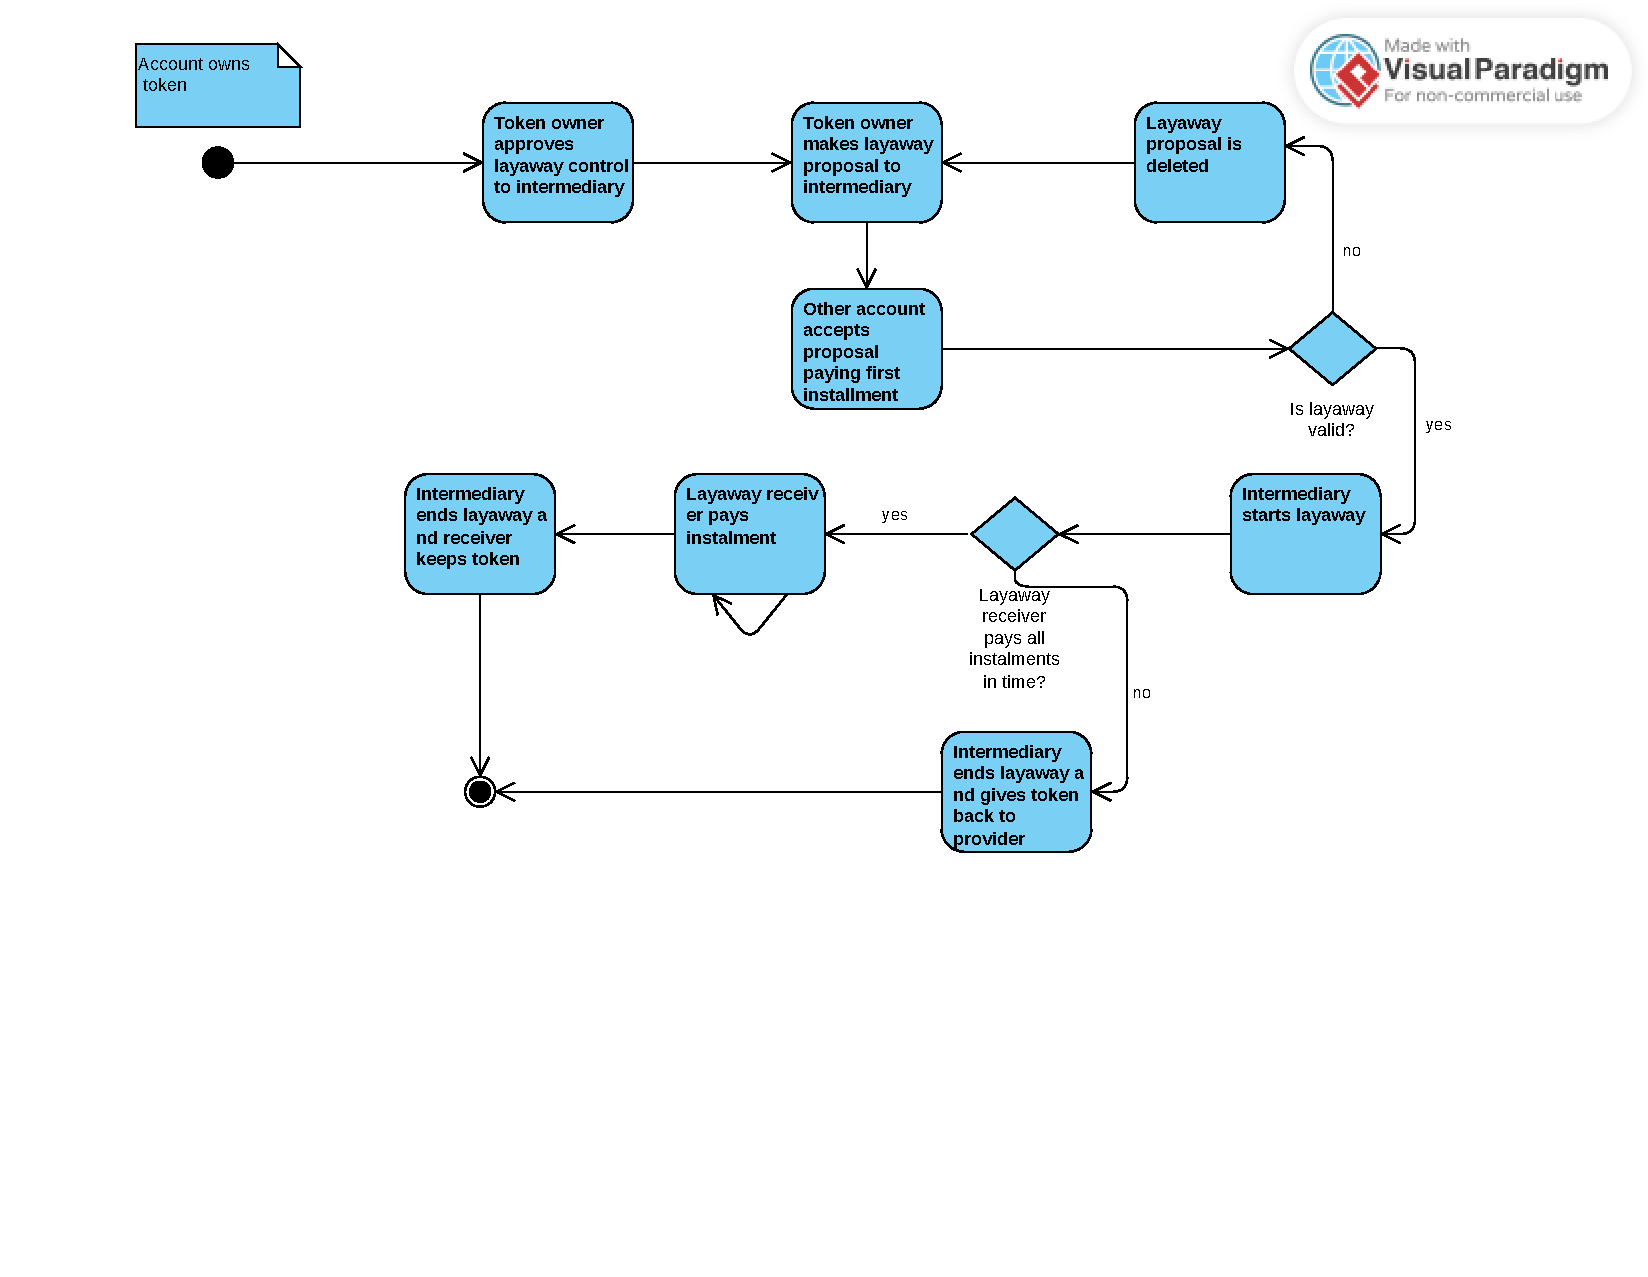
\includepdf[pages=-]{activity_layaway.pdf}
%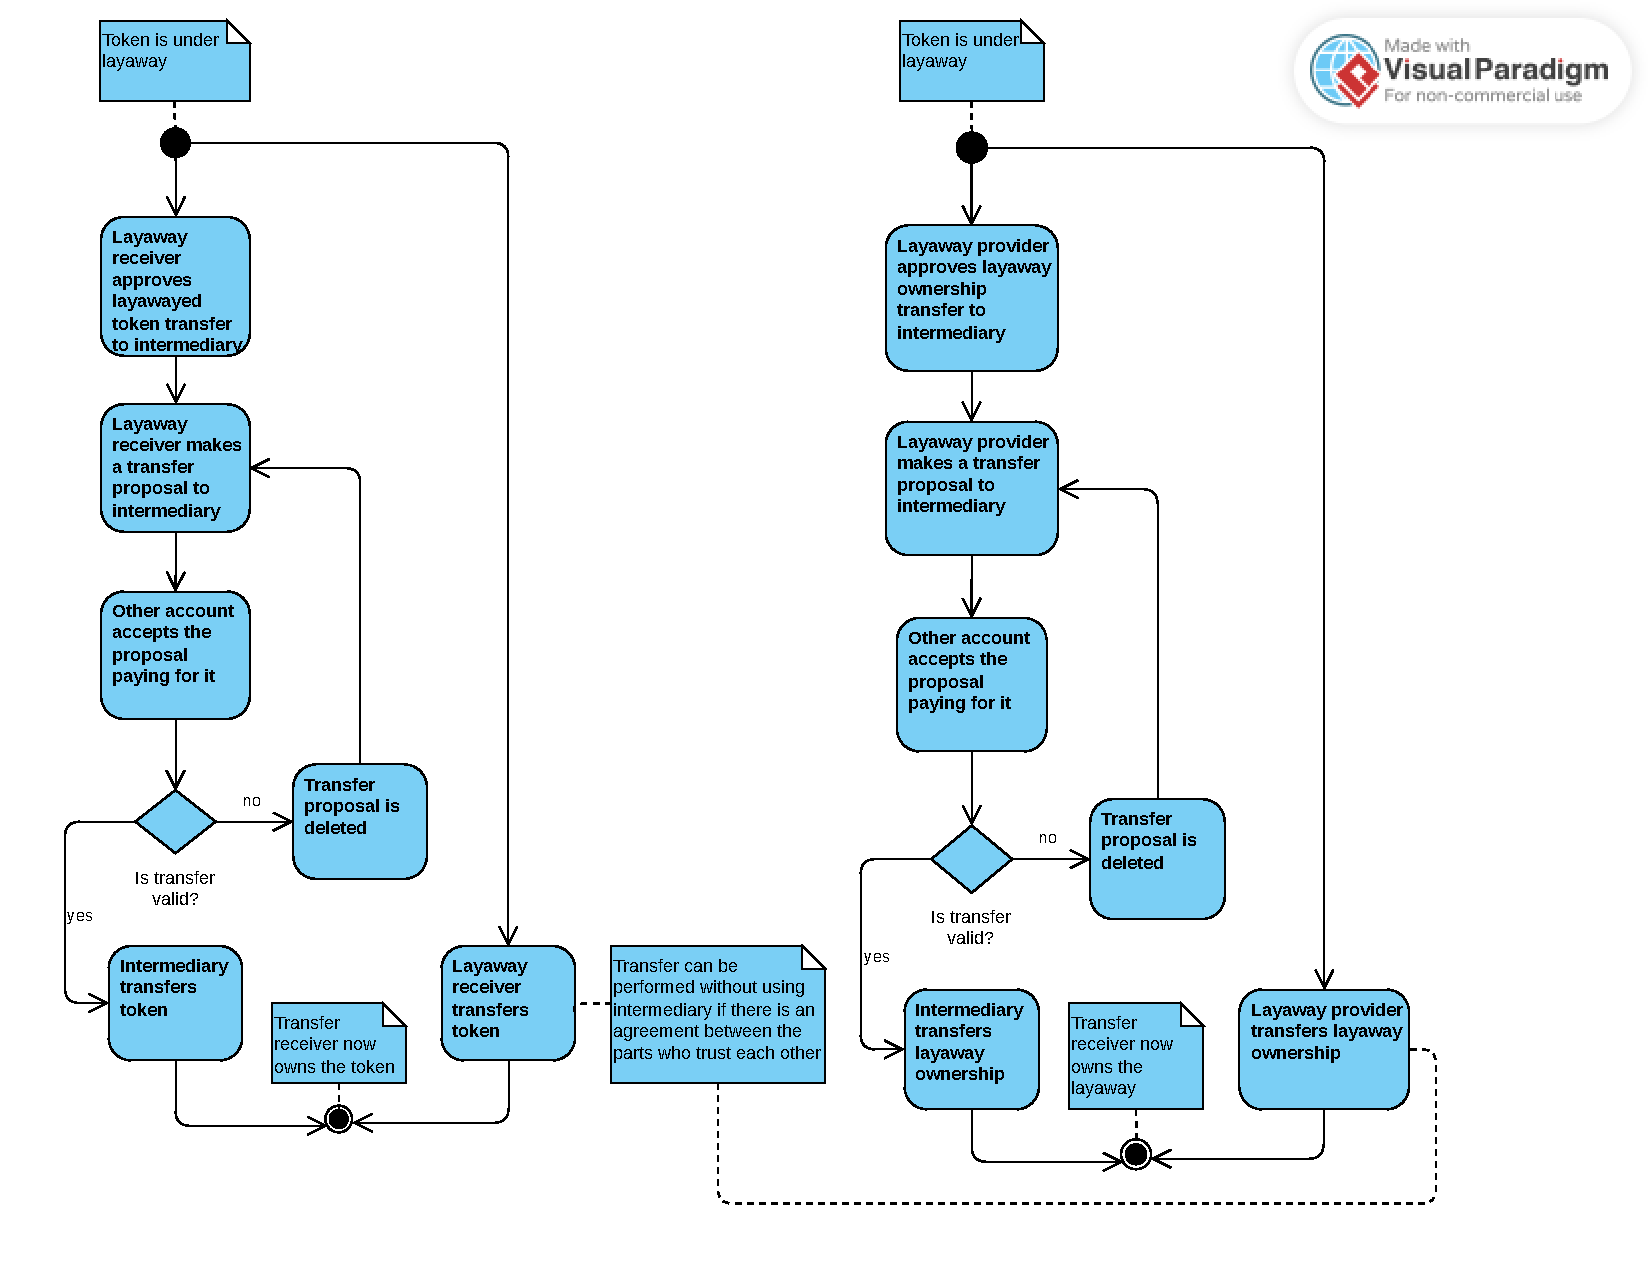
\includepdf[pages=-]{activity_layawayTransfer.pdf}
%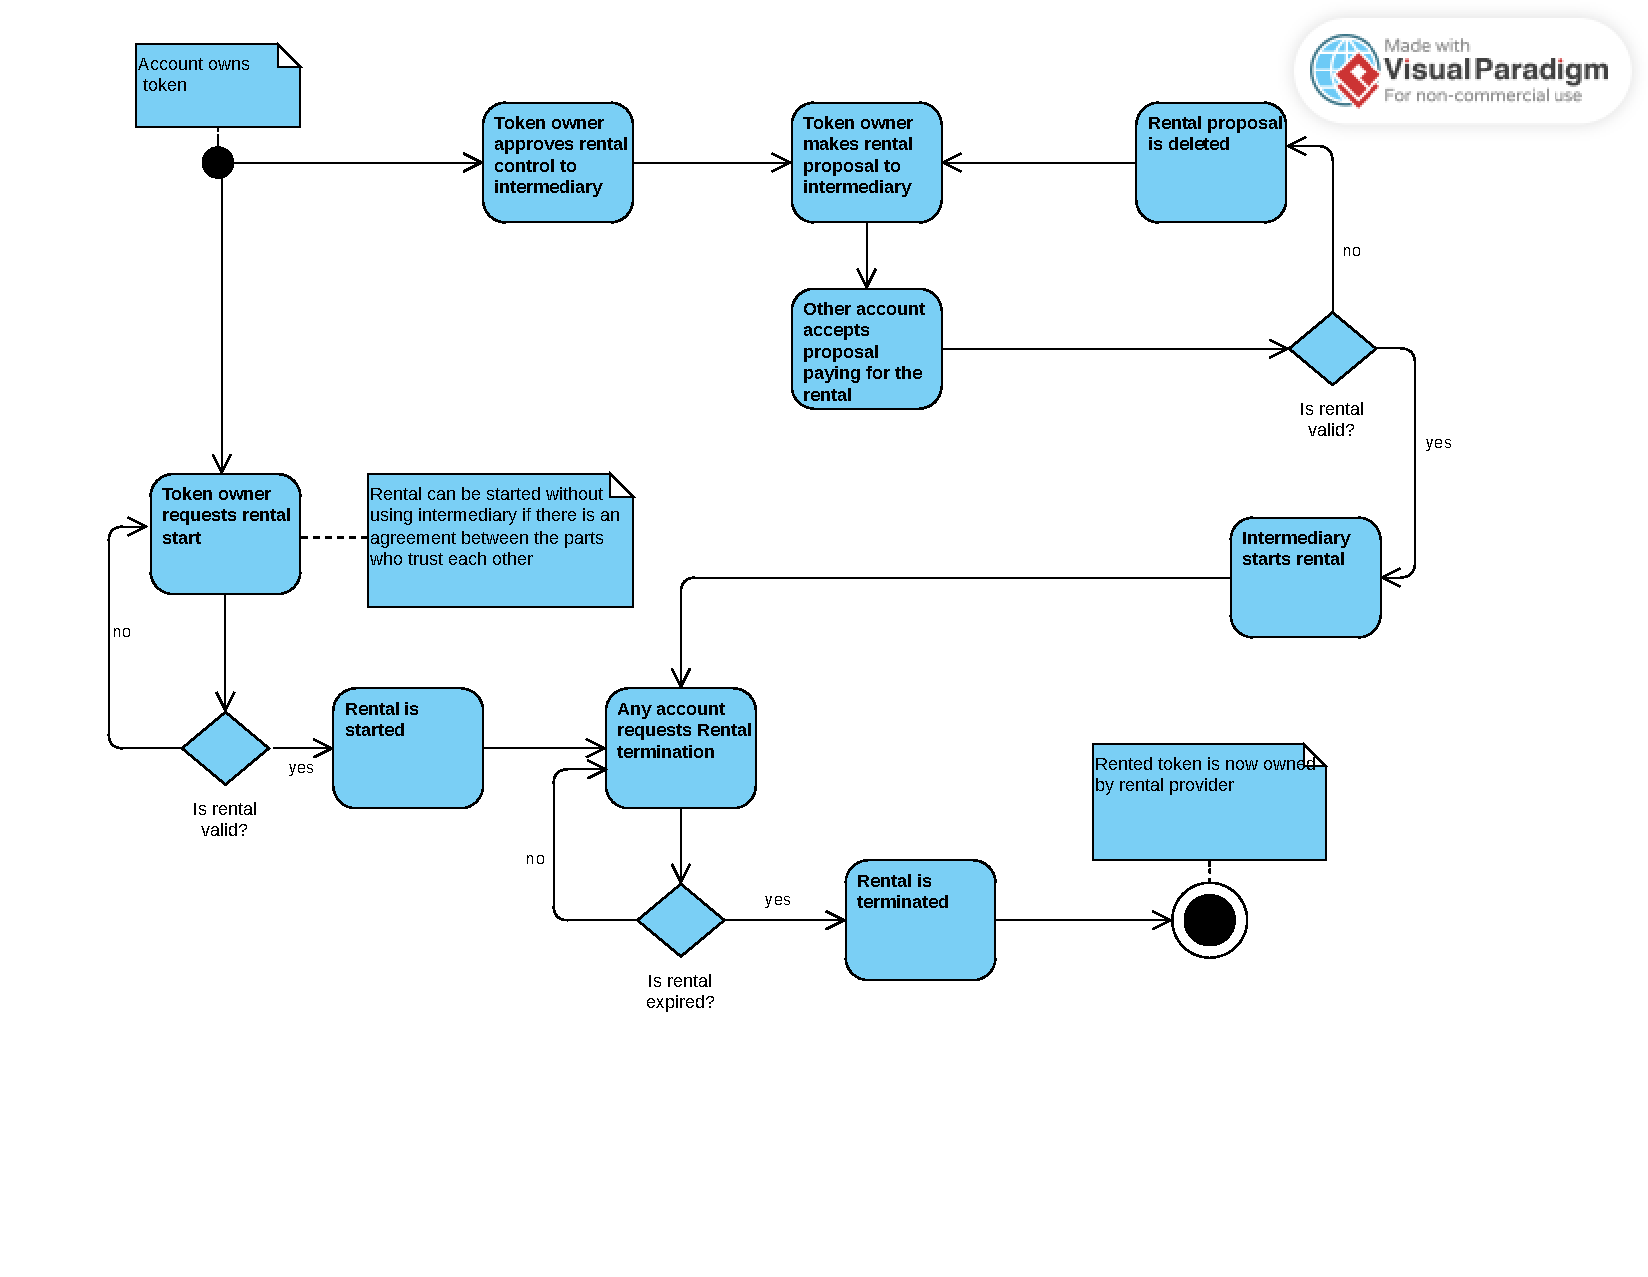
\includepdf[pages=-]{activity_rental.pdf}
%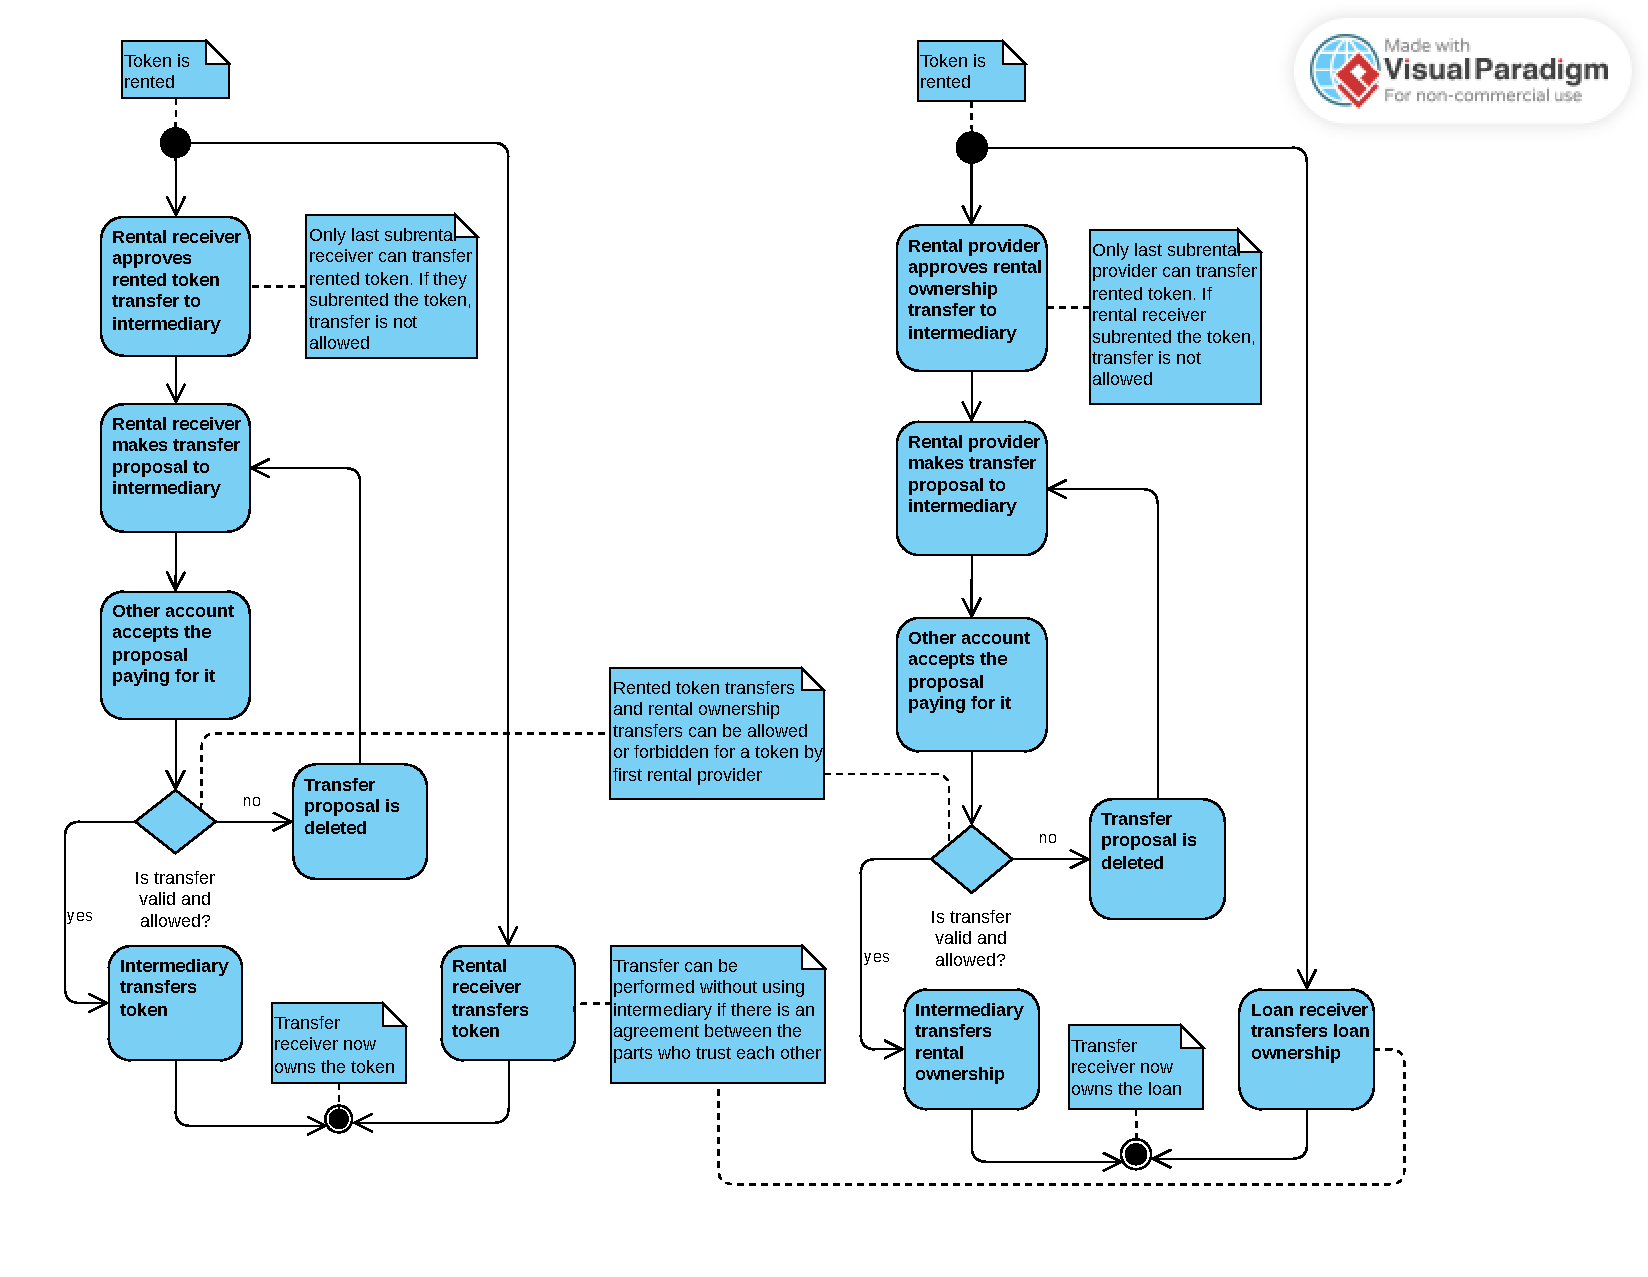
\includepdf[pages=-]{activity_rentalTransfer.pdf}
%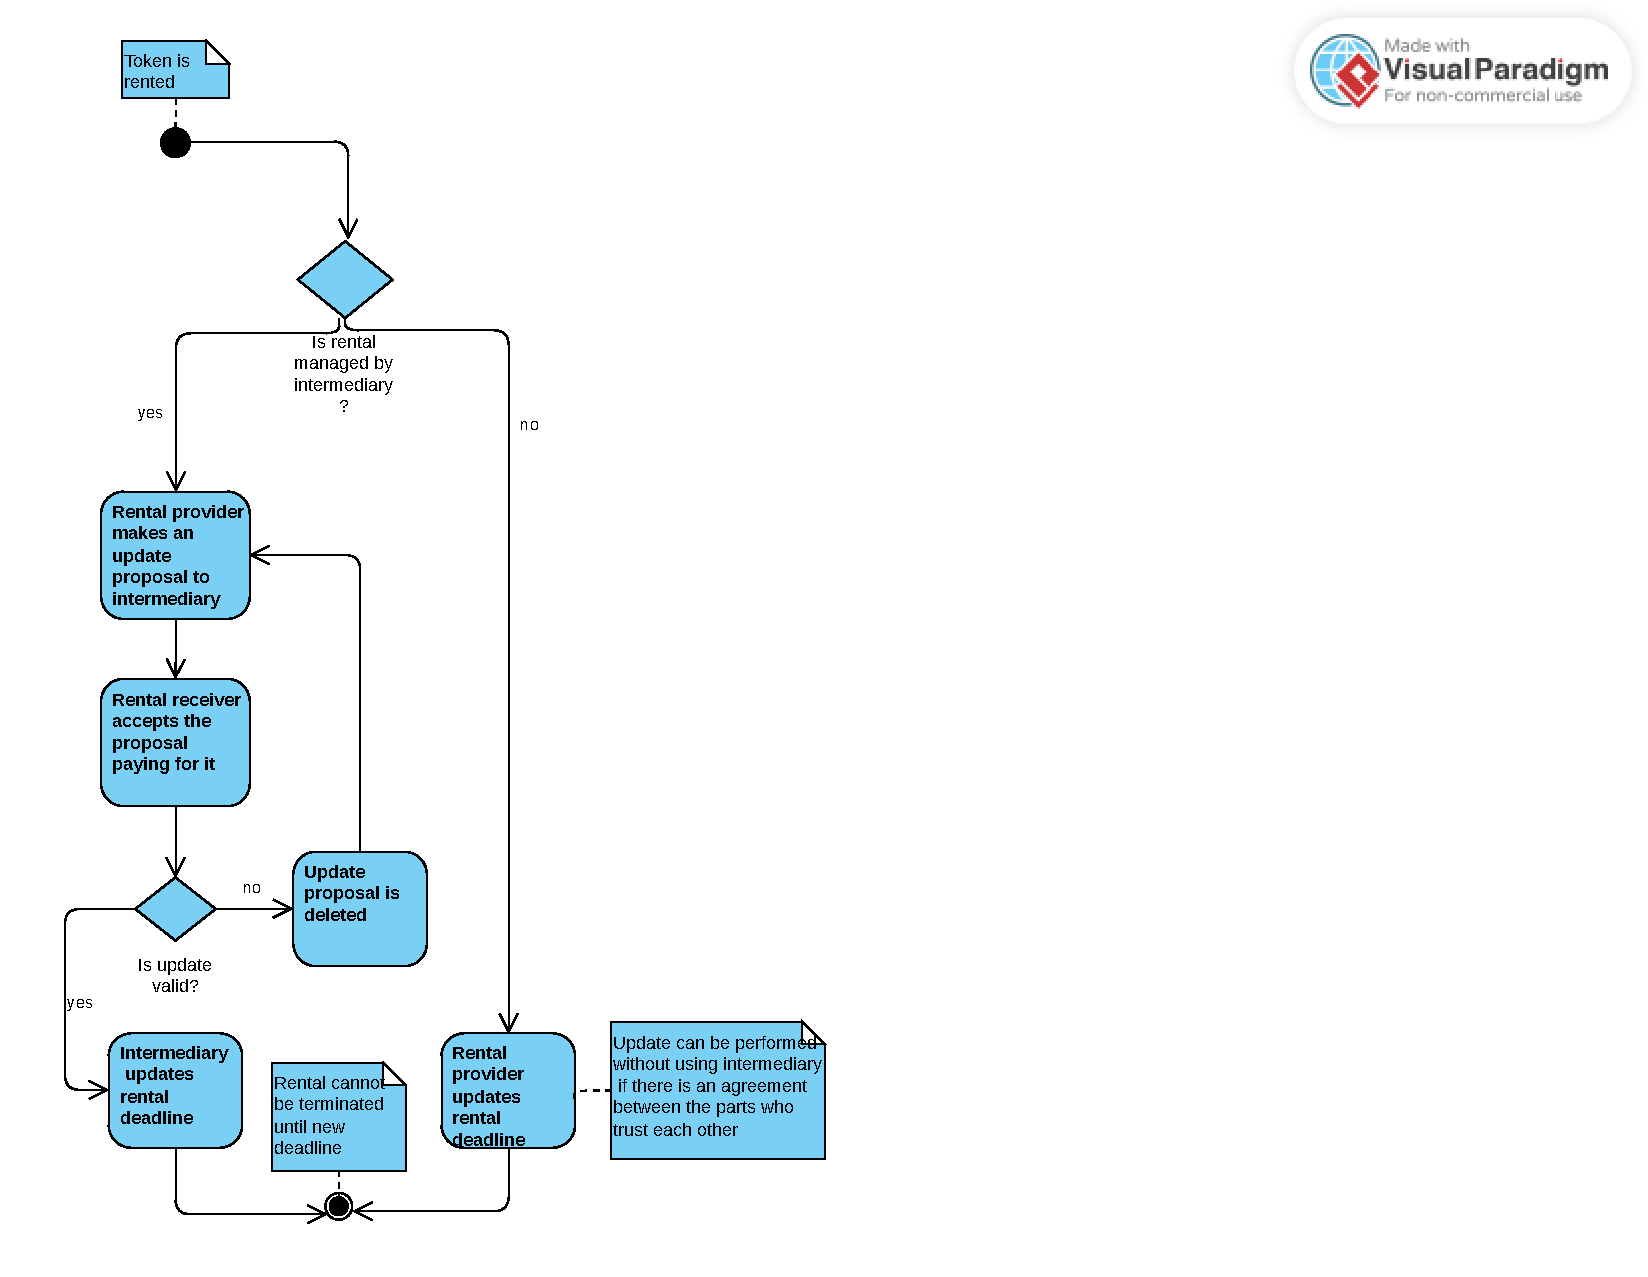
\includepdf[pages=-]{activity_rentalUpdate.pdf}
%\includepdf[pages=-]{activity_rentedTokenTransfer.pdf}
%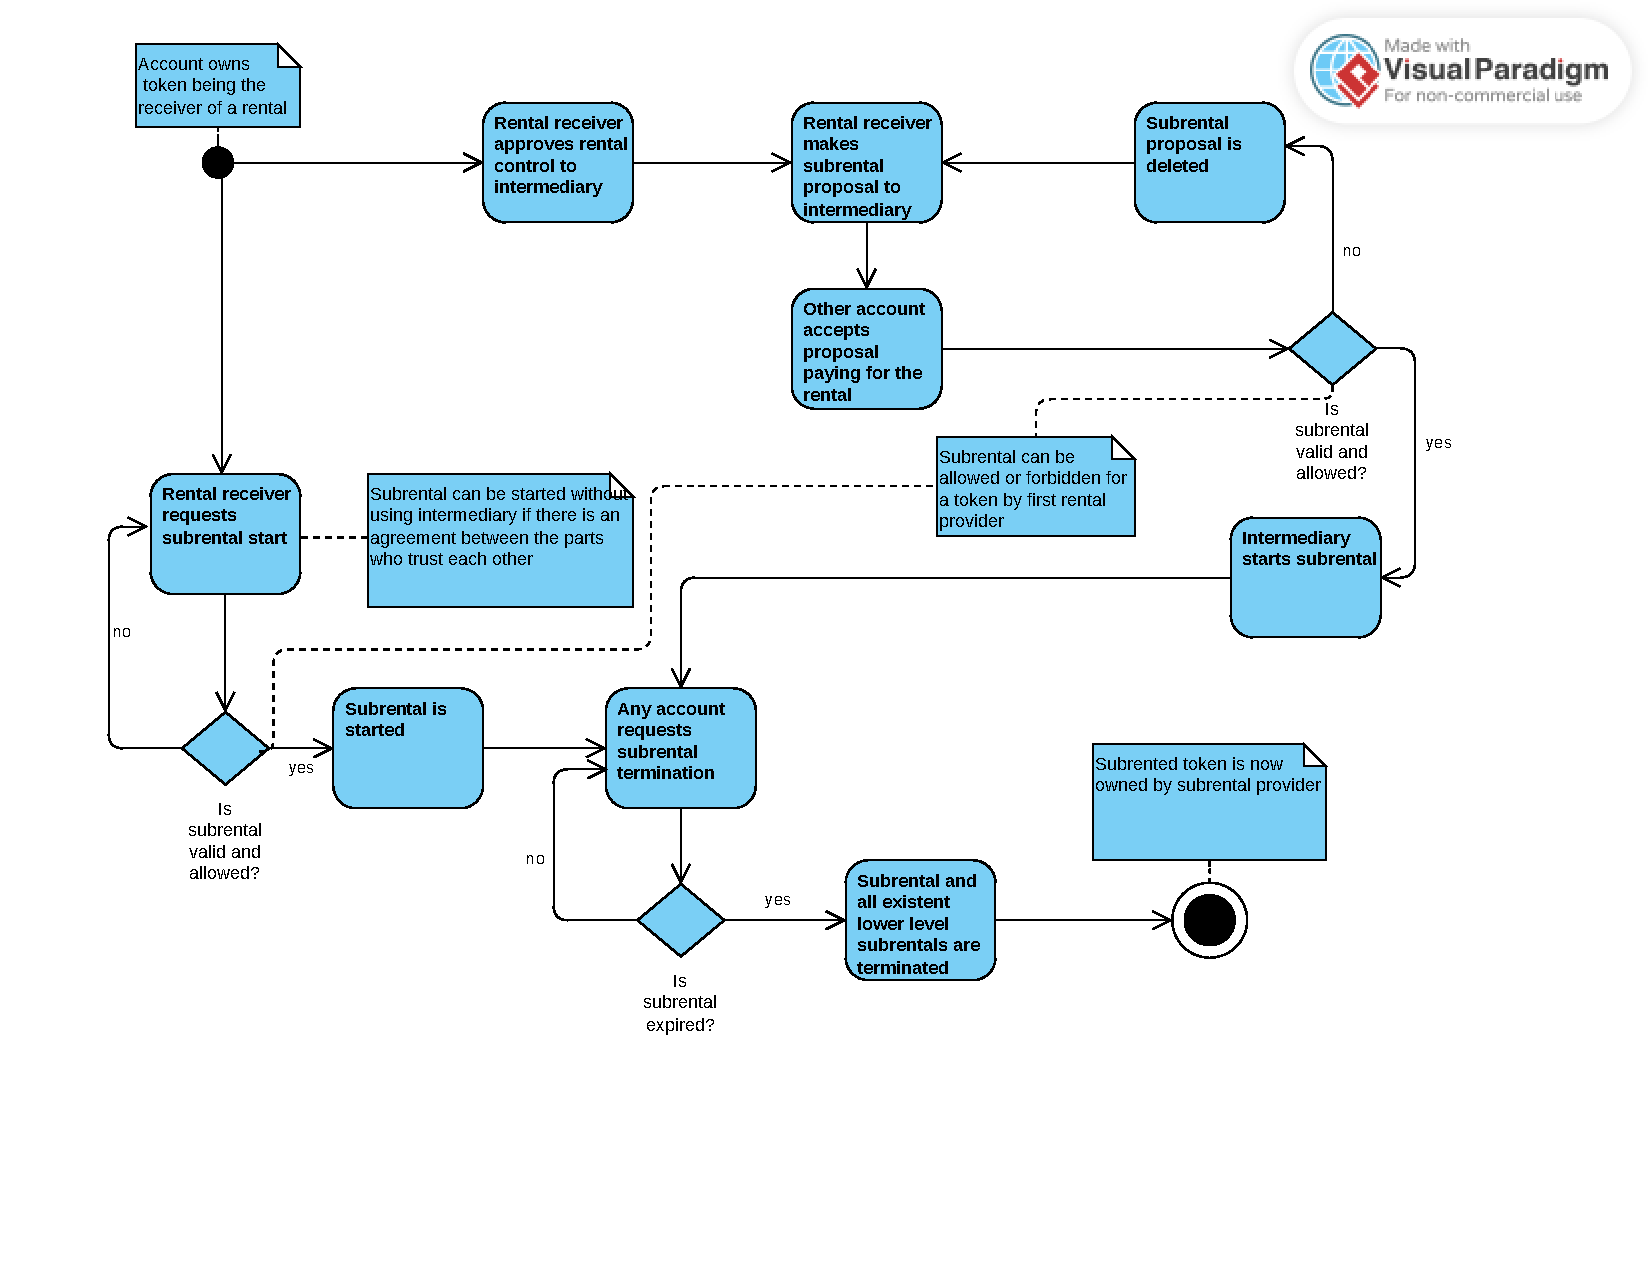
\includepdf[pages=-]{activity_subrental.pdf}
%\subsection{Sequence diagrams}

\section{Tests}
\label{sec:moons}
Lorem ipsum...



\chapter{Conclusions}
Lorem ipsum...

\backmatter
\phantomsection
\begin{thebibliography}{17}

\bibitem{ref:EIP4907}
Anders (@0xanders), Lance (@LanceSnow), Shrug <shrug@emojidao.org>, \textit{"ERC-4907: Rental NFT, an Extension of EIP-721,"} Ethereum Improvement Proposals, no. 4907, March 2022. [Online serial]. Available: \url{https://eips.ethereum.org/EIPS/eip-4907}.

\bibitem{ref:EIP721}
William Entriken (@fulldecent), Dieter Shirley <dete@axiomzen.co>, Jacob Evans <jacob@dekz.net>, Nastassia Sachs <nastassia.sachs@protonmail.com>, \textit{"ERC-721: Non-Fungible Token Standard"}, Ethereum Improvement Proposals, no. 721, January 2018. [Online serial]. Available: \url{https://eips.ethereum.org/EIPS/eip-721}.

\bibitem{ref:vera}
Vera Financial, \url{https://vera.financial}

\bibitem{ref:teller}
Teller Finance, \url{https://teller.org}

\bibitem{ref:supermojo}
Supermojo, \url{https://supermojo.com}

\bibitem{ref:eso}
European Southern Observatory, \url{http://www.eso.org}

\bibitem{ref:science}
Cirasuolo M., et al., \textit{"MOONS Science Report"}, MOONS Document Number: VLT-TRE-MON-14620-0001, Issue: $1.0$, $31^{\textup{st}}$ January $2013$


\end{thebibliography}

\end{document}